\documentclass[00-main.tex]{subfiles}

\begin{document}

\section{Validation by Simulation}\label{sec:simulations}
\subsection{Simulation Settings}\label{sec:simulation-settings}
The finite-sample performance of the pseudo-MLE $\hat{\bm\beta}^*$ \eqref{eq:beta_}, equivalently $\hat{\bm\theta}^*$ without covariates,  and the covariance estimators $\widehat{V}_\text{AR}$--$\widehat{V}_\text{OP}$ \eqref{eq:V_ar}--\eqref{eq:V_op} was assessed via Monte Carlo simulations across three settings. In each setting, $b =$ 900 independent replications of a sequence of choice and reaction times $\bm{Y} = (Y_1, \dots, Y_n)$ of length $n =$ 1000 were simulated under the true density ($f_0$; \ref{eq:f_dep}) and fit under the working density ($f^*$; \ref{eq:f_ind}). Settings vary along two dimensions: specification ($f_0 = f^*$ or $f_0 \neq f^*$) and parameter structure (fixed or varying across trials), which together determine whether the information matrix equality $\mathcal{H}_{\bm\beta} = \mathscr{I}_{\bm\beta}$ holds and which covariance estimators are consistent (Section~\ref{sec:covariance-estimation}). The first two settings are correctly specified, the second additionally demonstrates modeling of nonstationarity through covariates, while the third tests robustness to unmodeled parameter variability and temporal dependence.

\begin{itemize}

    \item \emph{Correct specification, constant parameters} ($f_0 = f^*$): a baseline correctly specified setting with parameters fixed across trials ($\bm{\theta}_i = \bm{\theta}^*$, no covariates). Decision outcomes are $iid$, the information matrix equality holds, and all four covariance estimators are expected to be consistent.

    \item \emph{Correct specification, trending decision boundary} ($f_0 = f^*$): a correctly specified setting where the decision boundary increases linearly from $0.8\beta_a$ to $1.2\beta_a$ over the session, with midpoint value $\beta_a = 0.63$, while all other parameters are held constant. The information matrix equality holds, and all four estimators are expected to be consistent. This setting demonstrates two capabilities of the pseudo-MLE: modeling DDM parameters as functions of covariates (Section~\ref{sec:covariates}), and explicitly accounting for nonstationary parameter trends with measured covariates.

    \item \emph{Misspecification and temporal dependence} ($f_0 \neq f^*$): a misspecified setting where $a$ is fixed and $t_0,v,z$ follow independent stationary two-state Markov chains, but all four parameters are estimated as constants. This constitutes misspecification of types (i) and (iii) (Section~\ref{sec:misspecification}). Only $\widehat{V}_\text{AR}$ accounts for both marginal misspecification and serial dependence; $\widehat{V}_\text{MR}$ addresses only the former.

\end{itemize}

Parameter centers were taken from \citet{matzke_psychological_2009} (Table~3 Means), rescaled to the present implementation: $\bar{a} = 0.63$, $\bar{t}_0 = 0.435$, $\bar{v} = 2.23$, $\bar{z} = 0.008$. Under correct specification, these serve as the true constant parameters, with $\bar{a}$ instead serving as the midpoint value $\beta_a$ for the trending boundary. The third setting is an illustrative robustness stress test: $a=0.63$, while $t_0 \in \{0.375,0.495\}$ seconds, $v \in \{0.90,3.56\}$, and $z \in \{-0.592,0.608\}$. Each chain starts in its equal-probability stationary distribution and remains in its current state with probability 0.85 (lag-one correlation 0.70). Outcomes are conditionally independent given these states, and each replication draws fresh chains and outcomes. The variability amplitudes were chosen in pilot simulations to illustrate marginal misspecification and temporal dependence, rather than to represent empirical parameter ranges. The pseudo-true parameters $\bm\theta^*$ need not equal the generating centers; they were determined independently by numerically integrating the expected working log-likelihood over the eight equally weighted stationary components. Empirical standard deviations and pairwise correlations across replications served as references for evaluating the covariance estimators.

\subsection{Simulation Results}

\subsubsection{Correct specification, constant parameters}
Simulations with constant parameters (Figure~\ref{fig:sim_constant}A,B) serve as a baseline for correct specification ($f_0 = f^*$). Point estimates (A; diagonals) are unbiased, meaning the sampling distributions are centered on the true parameters. Pairwise correlations (A; off-diagonals) are positive for $(a, v)$ and $(t_0, z)$, negative for $(a, t_0)$, $(t_0, v)$, and $(v, z)$, and near zero for $(a, z)$. Analytic standard error estimates (B; diagonals) are mostly unbiased except the non-robust estimators ($\widehat{V}_\text{SH}$, $\widehat{V}_\text{OP}$) show a slight upward bias for $v$, and the robust estimators ($\widehat{V}_\text{AR}$, $\widehat{V}_\text{MR}$) a slight downward bias for $t_0$ and $z$. The robust estimators also exhibit higher sampling variance than the non-robust estimators, most notably relative to $\widehat{V}_\text{OP}$, which has the lowest variance overall. Analytic pairwise correlation estimates (B; off-diagonals) are generally unbiased, with slight downward biases for $(a, v)$, $(t_0, z)$, and $(v, z)$ across both robust and non-robust estimators.

\begin{SCfigure}[][!h]
    \centering
    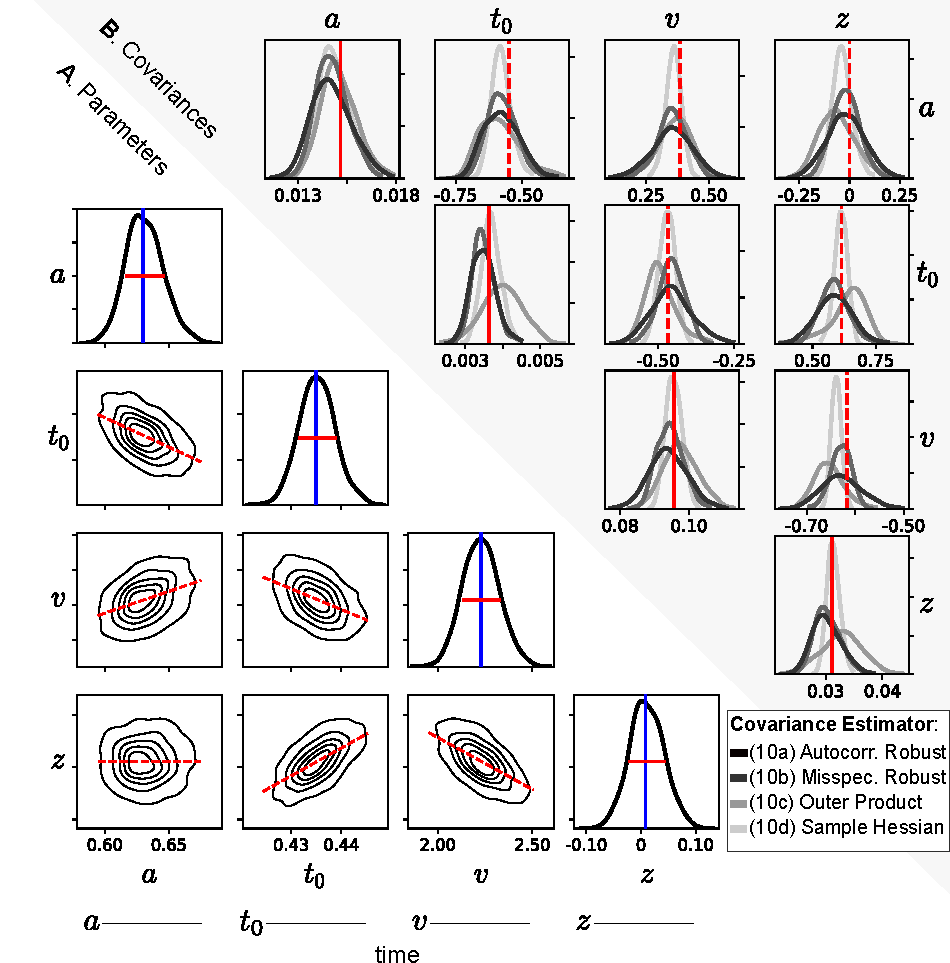
\includegraphics[width=0.5\textwidth]{docs/manuscript/figures/fig02-sim.pdf}
    \caption{\emph{Correct specification, constant parameters.}
    (A) \emph{Diagonals} show sampling distributions of $b=$ 900 point estimates ($\hat{\bm\theta}$; black density curves) around the true parameters ($\bm\theta$; blue vertical lines), where $\pm$ empirical standard deviations (red solid horizontal lines) are taken to be the true standard errors of the estimator. \emph{Off-diagonals} show bivariate sampling distributions of the point estimates (black density contours), where empirical correlations (red dashed lines) are taken to be the true correlations of the estimator. The schematic below each column indicates how the parameter varies over time (i.e., over the $n=$ 1000 trials), in this case indicating that all parameters are constant.
    (B) \emph{Diagonals} show sampling distributions of the $b=$ 900 analytic standard error estimates (i.e., square roots of the diagonal covariance elements; black=$\widehat{V}_\text{AR}$, dark gray = $\widehat{V}_\text{MR}$, gray = $\widehat{V}_\text{SH}$, light gray = $\widehat{V}_\text{OP}$) and the empirical standard errors from (A; solid red vertical lines). \emph{Off-diagonals} show analytic pairwise correlation estimates (black-gray density curves) and the empirical correlations from (A; red dashed vertical lines).}
    \label{fig:sim_constant}
\end{SCfigure}

\subsubsection{Correct specification, trending decision boundary}
Simulations where the decision boundary increases linearly over the session (Figure~\ref{fig:sim_linear}A,B) are also correctly specified ($f_0 = f^*$) because nonstationarity is explicitly modeled by the time covariate. Results are mostly comparable to the constant parameter simulation above (Figure~\ref{fig:sim_constant}). Point estimates (A; diagonals) remain approximately unbiased, now replacing the parameter $a$ with the midpoint value $\beta_a$. Pairwise correlations (A; off-diagonals) remain qualitatively similar. Analytic standard error estimates (B; diagonals) are mostly accurate: relative biases for $\widehat{V}_\text{SH}$ are within 3\%, while $\widehat{V}_\text{OP}$ shows an upward bias most notably for $t_0$ (11\%), and the robust estimators $\widehat{V}_\text{AR}$ and $\widehat{V}_\text{MR}$ show slight downward biases for $t_0$ and $z$ (3--4\%). Across parameters and covariance estimators, empirical coverage of nominal 95\% confidence intervals ranges from 92.7\% to 96.6\%. Analytic pairwise correlation estimates (B; off-diagonals) are generally close to the empirical correlations, with modest downward biases for $(\beta_a,t_0)$, $(\beta_a,z)$, and $(t_0,v)$, and for $(t_0,z)$ under the robust estimators. These results suggest that the covariance estimators remain mostly accurate when nonstationary trends are explicitly modeled.

\begin{SCfigure}[][h!]
    \centering
    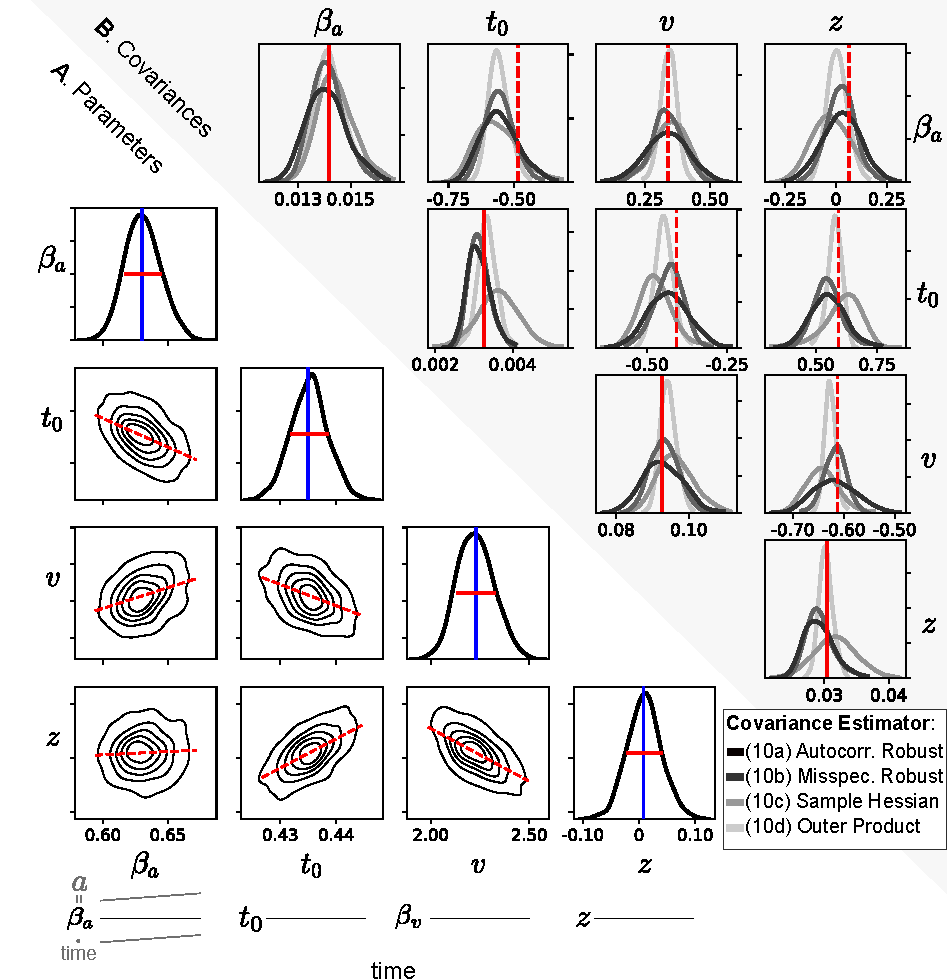
\includegraphics[width=0.5\textwidth]{docs/manuscript/figures/fig03-sim.pdf}
    \caption{\emph{Correct specification, trending decision boundary.}
    (A) As in Figure~\ref{fig:sim_constant}A, except the decision boundary $a_i$ increases linearly from $0.8\beta_a$ to $1.2\beta_a$ over the session (i.e., nonstationary), while its midpoint value $\beta_a = 0.63$ and all other parameters $t_0, v, z$ remain constant over time, such that the point estimates are for $\hat\beta_a$ instead of $\hat{a}$; as indicated by the schematic below the first column.
    (B) As in Figure~\ref{fig:sim_constant}B, except that $\beta_a$ replaces $a$.}
    \label{fig:sim_linear}
\end{SCfigure}

\subsubsection{Misspecification and temporal dependence}
Unmodeled persistent parameter variability (Figure~\ref{fig:sim_realistic}A,B) produces both marginal misspecification and serial dependence. Point estimates (A; diagonals) are close to the pseudo-true parameters $(a^*,t_0^*,v^*,z^*) \approx (0.575,0.339,1.267,-0.042)$, with a small upward bias for $t_0$ (0.00034 seconds, or 0.14 empirical standard deviations). Analytic standard errors (B; diagonals) distinguish the two robustness corrections: $\widehat{V}_\text{SH}$ and $\widehat{V}_\text{OP}$ overestimate standard errors for $t_0$ by 35\% and 105\%, respectively, while $\widehat{V}_\text{MR}$ reduces this bias to $-5$\%. However, $\widehat{V}_\text{MR}$ still underestimates standard errors for $v$ and $z$ by 26--27\%, compared with approximately 8\% for $\widehat{V}_\text{AR}$. Correlation estimates (B; off-diagonals) also improve overall with $\widehat{V}_\text{AR}$: for $(v,z)$, the empirical correlation is $-0.37$, compared with approximately $-0.60$ for the other estimators and $-0.45$ for $\widehat{V}_\text{AR}$. With six Bartlett-weighted lags at $n=1000$, $\widehat{V}_\text{AR}$ retains downward standard-error biases of 2--8\% across parameters; coverage of nominal 95\% intervals ranges from 92.2\% to 94.6\%.

\begin{SCfigure}[][h!]
    \centering
    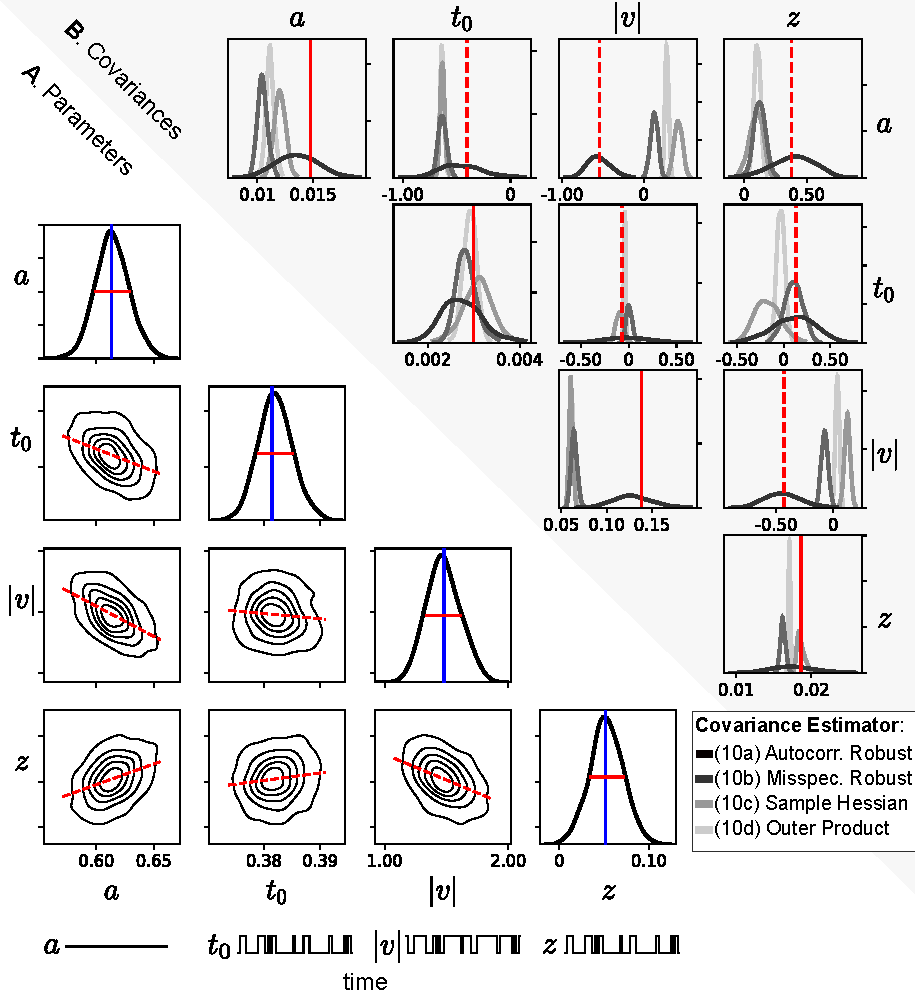
\includegraphics[width=0.5\textwidth]{docs/manuscript/figures/fig04-sim.pdf}
    \caption{\emph{Misspecification and temporal dependence.}
    (A) As in Figure~\ref{fig:sim_constant}A, except the blue vertical lines indicate pseudo-true parameters. The generating boundary $a$ is fixed, while $t_0$, $v$, and $z$ follow independent persistent two-state chains; all four parameters are estimated as constants.
    (B) As in Figure~\ref{fig:sim_constant}B. Only black=$\widehat{V}_\text{AR}$ accounts for both misspecification and serial dependence; dark gray=$\widehat{V}_\text{MR}$ corrects only marginal misspecification.}
    \label{fig:sim_realistic}
\end{SCfigure}

Overall, point estimates recovered the true or pseudo-true parameters, while autocorrelation-robust covariances improved uncertainty estimates under unmodeled variability and temporal dependence. Residual finite-sample bias cautions against assuming exact nominal coverage.

\end{document}
